\chapter{Система квантового распределения ключа на боковых частотах с применением обратной связи}\label{ch:ch2}
\section*{Система квантового распределения ключа на боковых частотах}
Одной из существующих реализаций систем квантового распределения ключа является реализация на боковых частотах, предложенная Юрием Тарасовичем Мазуренко. 
В отличии от других систем квантового распределения ключа, где лазерное излучение ослабляется до уровня мощности менее 1 фотона в импульсе, в системе квантового распределения ключа на боковых частотах (КРКБЧ) генерируются квантовые состояния на дополнительных оптических каналах, которые получаются в результате модулирования 
оптического лазерного излучения переменным электрическим сигналом с помощью электро-оптического модулятора на основе кристалла ниобата лития.
Такая реализация системы квантового распределения ключа дает преимущества в виде
\begin{enumerate}
    \item Устойчиовсть ко внешним воздействиям в виде колебаний волоконно-оптического тракта, которые изменяют поляризацию квантовых состояний случайным образом.
    \item Возможность реализации частотного мультиплексирования на одной оптической несущей частоте для повышения инфомрационной емкости канала или для повышения его секретности за счет случайного выбора частоты для измерений квантовых состояний.
    \item Совместимость с текущими волоконно-оптическими линиями связи за счет применения стандартной элементной-компонентной базы. 
\end{enumerate}
Эти преимущества выделяют систему квантового распределения ключа на поднесущих частотах среди остальных.
\subsection*{Принцип работы системы КРКБЧ}
Установка КРКБЧ работает следующим образом. Полупроводниковый лазер с рабочей длиной волны генерирует излучение на длине волны 1550 нм. Это излучение прередается по волоконно-оптическому тракту с сохранением поляризации на фазовый модулятор.
На электрический же вход электо-оптического модулятора подается радиосигнал, сформированный генератором. В качестве генератора выступает I/Q генератор, который на выходе выдает частоту 4.8 ГГц с фазовым кодированием.
Эти фазовые сдвиги определяют какое квантовое состояние кодирует Алиса в свои состояния. Значения данных фазовых свдигов соответствуют значениям {0, 90, 180, 270} градусов. 
В результате взаимодействия электрического и оптического сигнала внутри кристалла, на выходе модулятора в оптическом сигнале появляются дополнительные гармоники. Их частота будет равна $\omega - \Omega$ и $\omega + \Omega$, где $\omega$ - частота излучения лазера, $\Omega$ - частота модуляции.
Полученный в результате сигнал попадает на модулятор интенсивности на основе кристалла ниобата лития. Данно устройство создает импульсы из непрерывного излучения, сгенерированного лазером. Это необходимо для того, чтобы было возможно регулировать время прихода одиночного фотона на детектор одиночных фотонов, режим работы которого будет описан далее.
Приготовленные импульсы попадают на аттенюатор оптической мощности (ПОА), который вносит затухание в пришедший сигнал до такого уровня, что на поднесущих частотах должна быть мощность, равная средней мощности, которая соответствует среднему числу фотонов меньше единицы.
При этом на несущей частоте допускается использование мощности больше 1 фотона в среднем, так как сигнал на этой частоте не используется для распределения секретного ключа.
Сгенерированные квантовые состояния передаются в блок приемника по стандартной волоконно-оптической линии связи, построенной с помощью одномодового волокна. 
Пройдя ВОЛС сигнал попадает на блок приемника. 
При прохождении сигнала по такой линии связи, поляризация прошедшего состояния изменяется на случайную, что приводит к негативным последствиям. 
\section{Метод оптической инжекции}\label{sec:ch2/sec1}
Для систем квантового распределения ключа необходимы стабильные источники излучение с фиксированной длиной волны и без нелинейных эффектов в виде чирпа. Некачественные источники лазерного излучения привдоят к нарушению интерфереционной картины в случае протоколов MDI или же снижению скорости генерации секретного ключа и уменьшения дальности его передачи в протоколах BB84 с применением состояний ловушек. Одним из активно развивающихся решений этой проблемы является метод фазовой синхронизации с помощью оптической инжекции. 
\newline Полупроводниковые лазеры  на основе кристалла InGaAs имеют выходное зеркало, которое пропускает больше 50\% излучения. Благодаря такому коэффициенту пропускания, такие лазеры подвержены внешнему оптическому воздействию, которое зачастую является нежелательным из-за возможного образования паразитной обратной связи. Однако эту прозрачность можно использовать во благо для реализации оптической инжекции. Этот метод предлагает использование второго лазера, излучение которого попадает в резонатор другого лазера, образуя пару ведущий - ведомый. В результат этого выходное излучение ведомого лазера меняется под действием излучения ведущего источника. К плюсам метода оптической инжекции можно отнести следующее
\begin{enumerate}
    \item Применение оптической инжекции улучшает форму спектра выходного излучения, уменьшая дополнительные гармоники.
    \item Уменьшает возникающие в кристалле нелинейные процессы, негативно влияющие на частотный составл выходного излучения
    \item Улучшает форму выходных импульсов за счет подавления релаксационных колебаний и стабилизации выходной частоты
    \item Стабилизация амплитуды и длительности импульсов
\end{enumerate}
Данные эффекты положительно сказываются на качестве выходного излучения и, как следствие, положительно влияют на характеристики систем квантвого распределения ключа, в которых они используются.
\subsection{Математическая модель оптической инжекции}
Система уравнений описывающих излучение ведомого лазера:
\begin{equation}\label{eq:systemForMaster}
	\begin{split}
		\dot{Q}^{\text{м}} &= (G^{\text{м}} - 1)\frac{Q^{\text{м}}}{{{\tau_{\text{ф}}^{\text{м}}}}}+ C_{\text{сп}}^{\text{м}} R_{\text{сп}}^{\text{м}} +F_Q^{\text{м}}, \\ 
		\dot{\varphi}^{\text{м}} &= \frac{\alpha^{\text{м}} }{{2{\tau_{\text{ф}}^{\text{м}}}}}(G_{\text{лин}}^{\text{м}} - 1)+F_\varphi^{\text{м}},\\
		\dot{N} ^{\text{м}} &= \frac{I^{\text{м}}}{e} - \frac{N^{\text{м}}}{{{\tau _e^{\text{м}}}}} - \frac{{G^{\text{м}}Q^{\text{м}}}}{{\Gamma^{\text{м}} {\tau_{\text{ф}}^{\text{м}}}}}+F_N^{\text{м}},	
	\end{split}
\end{equation}
и связанную систему для ведомого лазера:
\begin{equation}\label{eq:systemForSlave}
	\boxed{	\begin{split}
			\dot{Q} &= (G - 1)\frac{Q}{{{\tau_{\text{ф}}}}}+ C_{\text{сп}} R_{\text{сп}}+ \\
			&
			+ 2{\kappa_{\text{и}}}\sqrt {Q^{\text{м}}Q} \cos (\Delta \omega_{\text{и}} t + {\varphi ^{\text{м}}} - \varphi )+F_Q, \\ 
			\dot{\varphi} &= \frac{\alpha }{{2{\tau_{\text{ф}}}}}(G_{\text{лин}} - 1)+ \\
			&+ {\kappa_{\text{и}}}\sqrt {\frac{{Q^{\text{м}}}}{Q}} \sin (\Delta \omega_{\text{и}} t + {\varphi^{\text{м}}} - \varphi )+F_\varphi,\\
			\dot{N} &= \frac{I}{e} - \frac{N}{{{\tau _e}}} - \frac{{GQ}}{{\Gamma {\tau_{\text{ф}}}}}+F_N,
	\end{split}}
\end{equation}
где члены $C_{\text{сп}}^{\text{м}}R_{\text{сп}}^{\text{м}}$ и $C_{\text{сп}}R_{\text{сп}}$ описывают вклад спонтанного излучения (см. раздел \ref{sec:inclofspontemission}), а $F_Q^{\text{м}} $, $F_\varphi^{\text{м}}$, $F_N^{\text{м}}$ и $F_Q$, $F_\varphi$, $F_N$ -- ланжевеновские силы для ведущего и ведомого лазеров соответственно.
\section{Измерение диапазона фазовой синхронизации двух когерентных источников излучения}\label{sec:ch2/sect2}
При методе оптической инжекции необходимо учитывать то, что два лазера необходимо настроить таким образом, чтобы их излучение синхронизировалось по фазе. Для этого необходимо учитывать то, что существует полоса синхронизации, которая определяется как 
\begin{equation}\label{eq:DbigOmega}
	\Delta \Omega=\Delta \omega_{\text{синх}} \sin(\varphi_{\text{синх}}-\psi),
\end{equation}
где $\Delta \omega_{\text{синх}}$ определяется как
\begin{equation}\label{eq:lockingBandwidth}
	\Delta \omega_{\text{синх}} = z\sqrt{1+\alpha^2(1+2\gamma_Q Q_\text{с})},
\end{equation}
и где мы ввели обозначение
\begin{equation}\label{eq:z}
	z=\kappa_{\text{и}}\sqrt{Q^{\text{м}}_\text{с}/Q_\text{с}}.
\end{equation}

Уравнение \eqref{eq:DbigOmega} накладывает первое ограничение на полосу синхронизации, которое можно записать следующим образом:
\begin{equation}\label{eq:symLockingBandwidth}
	\lvert \Delta \Omega \rvert \le\Delta \omega_{\text{синх}}.
\end{equation}
выражение \ref{eq:symLockingBandwidth} показывает, что необходимо подбирать частоты и мощности ведущего и ведомого лазера для их синхронизации. 
\newline Для этого используются исследуемые лазеры и оптичесский анализатор спектра. У ведущего лазера изменяется длина волны за счет изменения температуры кристалла, контролируемой управляющей электроникой через элемент Пельтье. Излучение лазера ведомого подключается через оптический циркулятор с сохранением поляризации для минимизиации потерь в волокне. Второй вход циркулятора же подключен к волоконному выводу лазера-ведомого, чтобы излучение из лазера-ведущего входило внутрь резонатора. Выходное излучение лазера-ведомого подается на второй выход циркулятора и проходит в третий его порт, где устанавливается оптический анализатор спектра, который измеряет характеристики пришедшего излучения.  В случае синхронизации, на анализаторе спектра возникает только одна длина волны лазера без изменений. Однако в случае разницы длин волн слишком большой, то будет наблюдаться несколько гармоник излучения, которые соответствуют длинам волн лазера-ведомого и лазера-ведущего. При некоторой комбинации длин волн, может также наблюдаться генерация нелинейных гармоник сигнала, сигнализирующих о том, что лазеры находятся в зоне нестабильной синхронизации. 
Таким образом подбирается оптимальное соотношение длин волн лазеров. Для дальнейшего изучения диапазона возможно использование перестараиваемого аттенюатора в волокнонном тракте лазера-ведущего для изменения соотношения мощностей лазера-ведущего и лазера-ведомого.
\section{Оптическая схема эксперимента для системы квантового распределения ключа на боковых частотах с применением метода оптической инжекции}\label{sec:ch2/sec3}
Для системы кватового распределения ключей на боковых частотах на непрерывных переменных с когерентным методом детектирования вопрос создания обратной связи и использования локального осциллятора на стороне приемника не изучался. В рамках данного раздела предлагается оптическая схема эксперимента по передаче фазово-кодированных сигналов по волоконно-оптической линии связи. Для регистрации фазово-кодированных сигналах на поднесущих гармониках применяется метод гетеродинного детектирования сигналов. Его суть заключается в том, чтобы закодированный сигнал на симметричном светоделителе проинтерферировал с опорным излучением локального осциллятора. Также излучение локального осциллятора, установленного в блоке получателя, выступает в роли лазера-ведущего для источника излучения, установленного в блоке отправителя. За счет этого достигается синхронизация длин волн излучения лазера-ведущего и лазера-ведомого, локального осциллятора и информационного лазера соответственно. Эта особенность позволяет не применять частотную подстройку источников излучения и упростить конечную систему.

\section{Описание экспериментальной установки}\label{sec:ch2/sect4}
Оптическая схема установки по экспериментальной передаче фазово-кодированных сигналов и применением гетеродинного метода детектирования и оптической инжекции на рисунке 
\begin{figure}
    \centering
    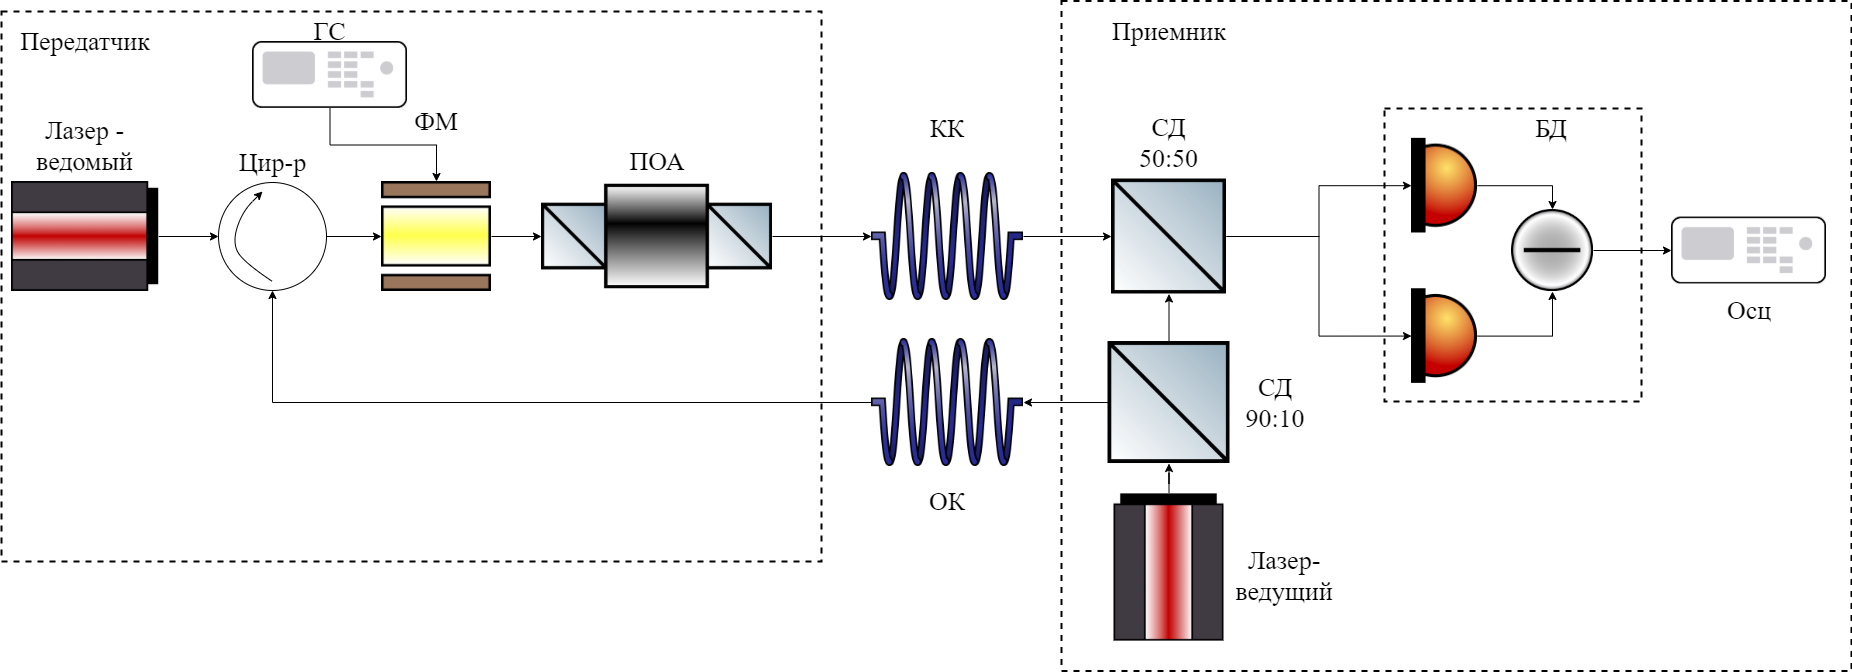
\includegraphics[width=\textwidth]{images/Схема с обратной связью новая 2 .png}
    \caption{Оптическая схема установки системы КРК на поднесущих гармониках с оптической инжекцией, где СД - светоделитель, ГС - генератор сигналов, ФМ - фазовый модулятор, ПОА - переменный оптический аттенюатор, КК - квантовый канал, ОК - открытый канал, Цир-р - циркулятор, БД - балансный детектор, Осц - осциллограф}
    \label{fig:feedback scheme ch2}
\end{figure}
Данная схема работаетследующим образом. Лазер-ведущий генерирует оптическое излучение, которое разделяется на 2 части светоделителем 90:10, 10 процентов которого по открытому каналу передаются на сторону передатчика в 1 порт оптического циркулятора. Во второй порт циркулятора подключен лазер передатчика. Такая схема подключения как раз создает оптическую инжекцию и частоты лазера передатчика и лазера локального осциллятора совпадают. Полученное излучение на стороне передатчика проходит фазовую модуляцию с помощью связки фазового модулятора и генератора сигналов произвольной формы на частоте 100 МГц. После этого подготовленный сигнал ослабляется с помощью переменного оптического аттенюатора. После этого излучение передается по квантовому каналу на сторону приемника. В приемнике принятный сигнал попадает на симметричный светоделитель с 2 входами и 2 выходами с коэффициентом деления 50:50. На второй же вход этого делителя попадает излучени ЛО, его 90 процентов после светоделителя. В итоге эти сигналы интерферируют и результат этой интерференции регистрируется балансным детектором. Так как длины волн информационного лазера и ЛО совпадают, то в результате интерференции они регистрируются как постоянный уровень напряжения, однако благодрая выносу фазово-кодированных состояний на поднесущие гармоники, то их интерференция с ЛО и дает результат в виде промежуточной частоты, которая равна частоте модуляции, применненой в Алисе. Эта частота на выходе балансного детектора осцифровывается с помощью осциллографа и в дальнейшем обрабатывается. 
\section{Полученные экспериментальные результаты}\label{sec:ch2/sect5}

В результате интерференции на выходе балансного детектора регистрируется промежуточная частота  равная $\omega + \Omega - F$, где $\omega$ - частота лазера Алисы, $\Omega$ - частота модуляции, F - частота ЛО. Благодаря применению оптической инжекции частоты ЛО и лазера Алисы совпадают, поэтому на выходе балансного детектора остается только гармоника на частоте модуляции, в которую и вносится фазовый свдиг для передачи информации. Этот сигнал изображен на рисунке \ref{fig:100 MHZ filt ch2}
\begin{figure}
    \centering
    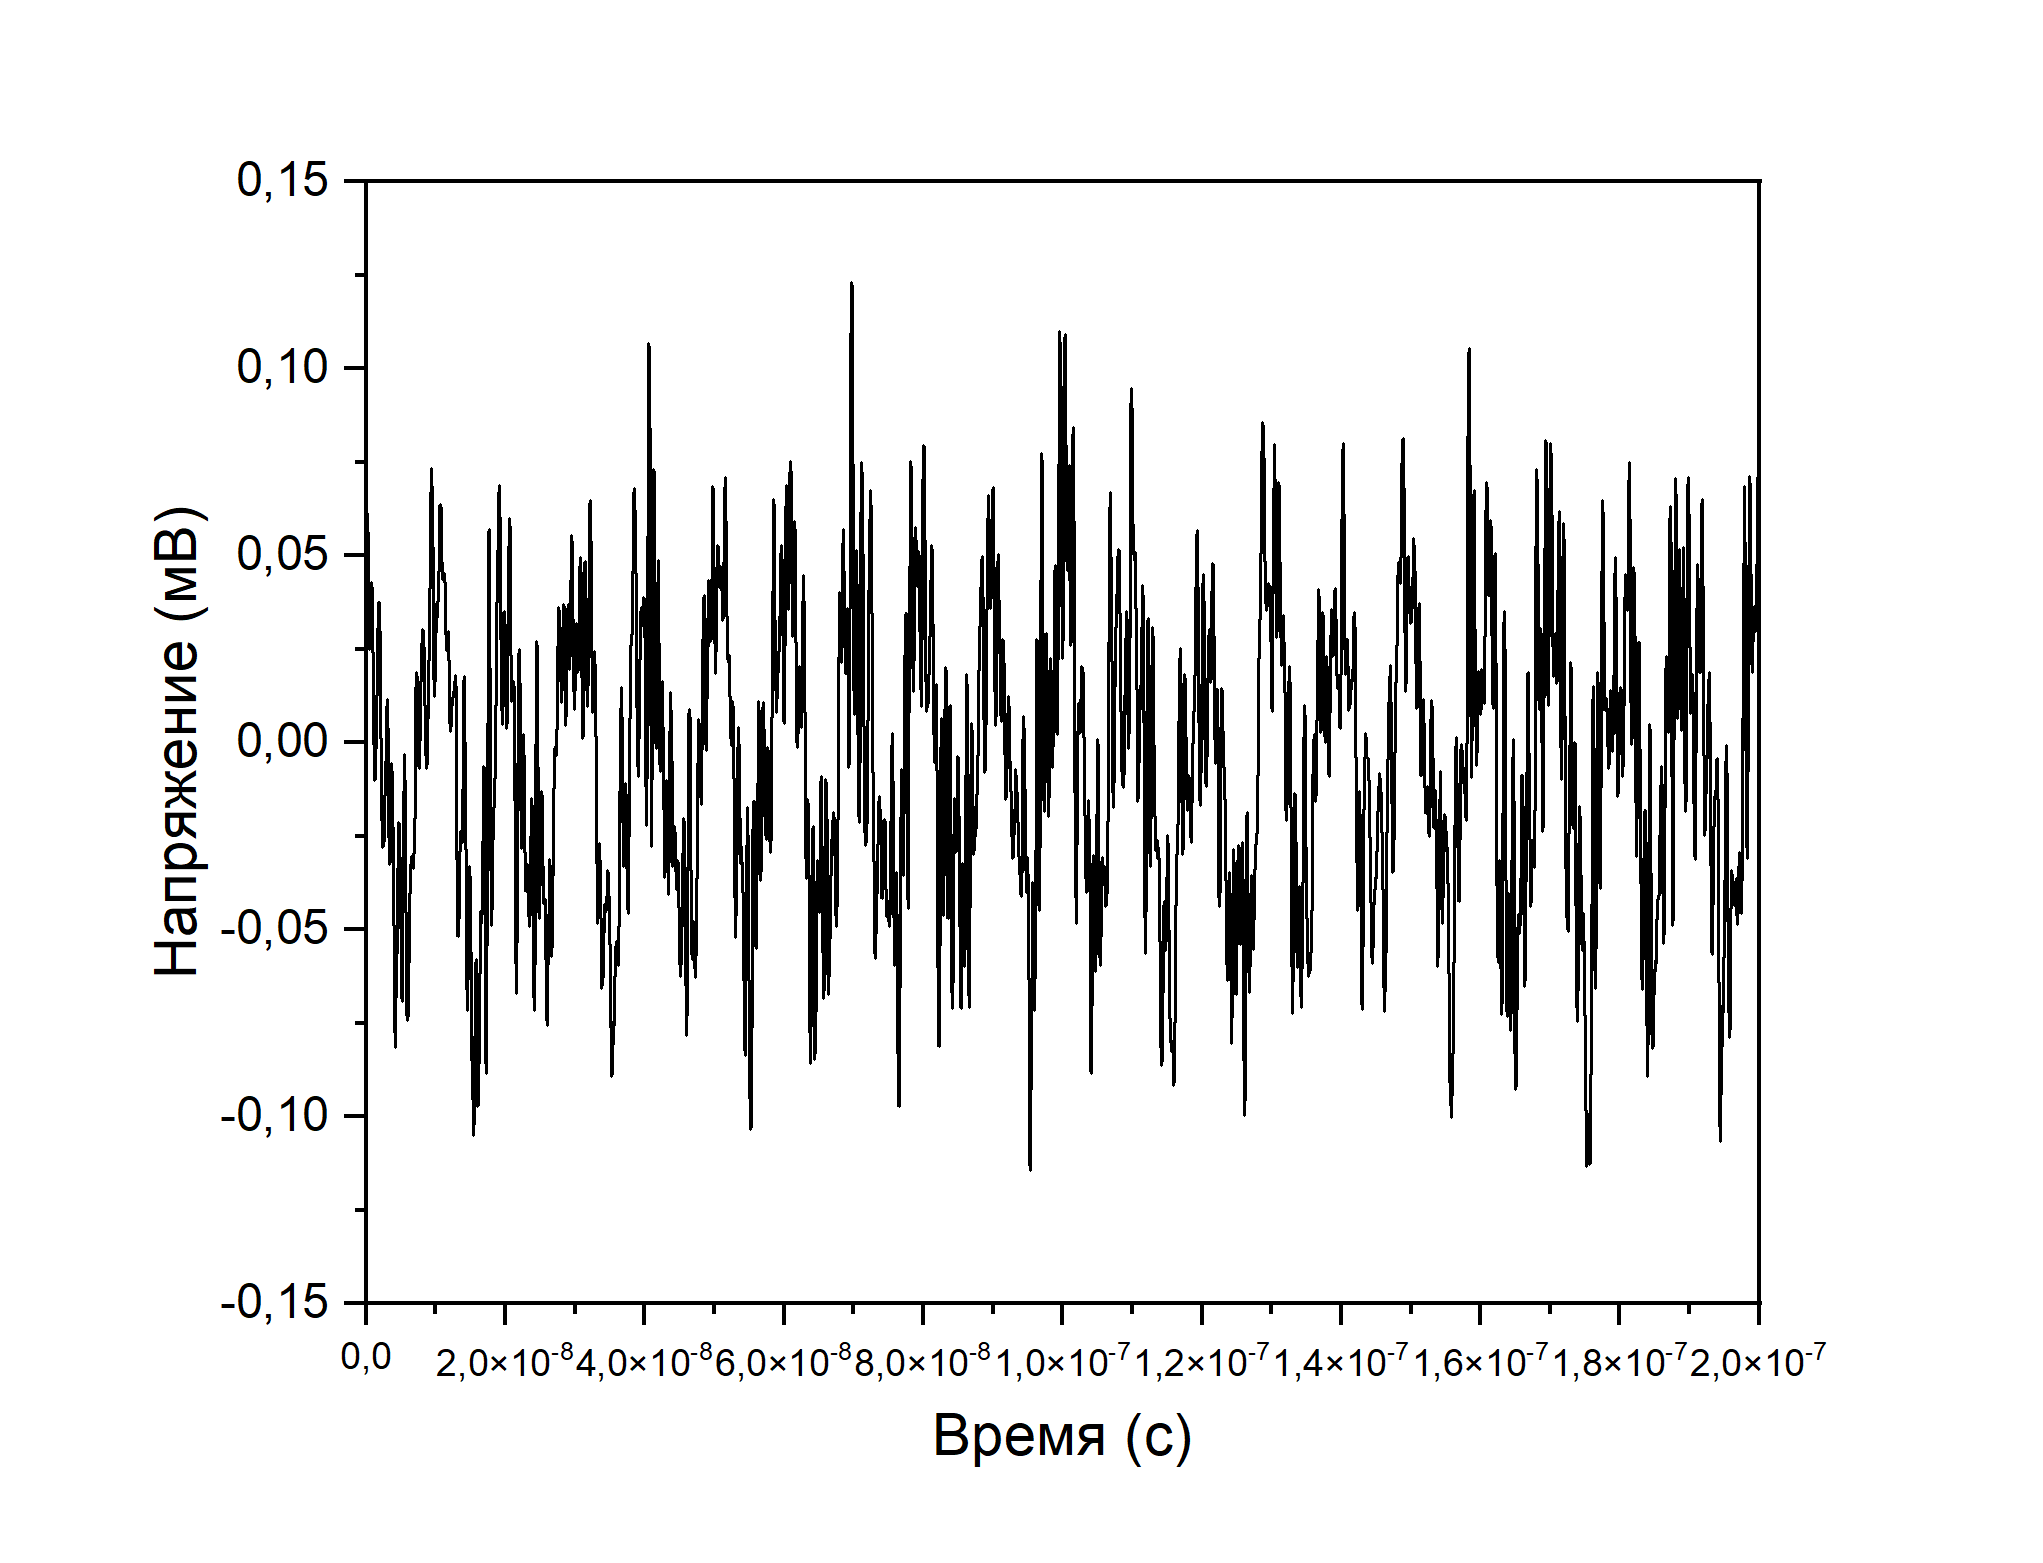
\includegraphics[width=\textwidth]{images/сигнал после бд с новыми шкалами.png}
    \caption{Выходной зашумленный сигнал на выходе балансного детектора.}
    \label{fig:100 MHZ filt ch2}
\end{figure}
На этом графике видна один гармонический сигнал в 100 МГц, в котором содержится информация о фазе, которую необходимо извлечь методами цифровой обработки сигналов. Для более точного измерения фазы сигнала, необходимо эту частоту отфильтровать от шума, который появлятеся из-за прохождения канала и собственных шумов балансоного детектора. Результат цифровой фильтрации сигнала с рисунка  \ref{fig:100 MHZ filt ch2} отображается ниже. 
\begin{figure}
    \centering
    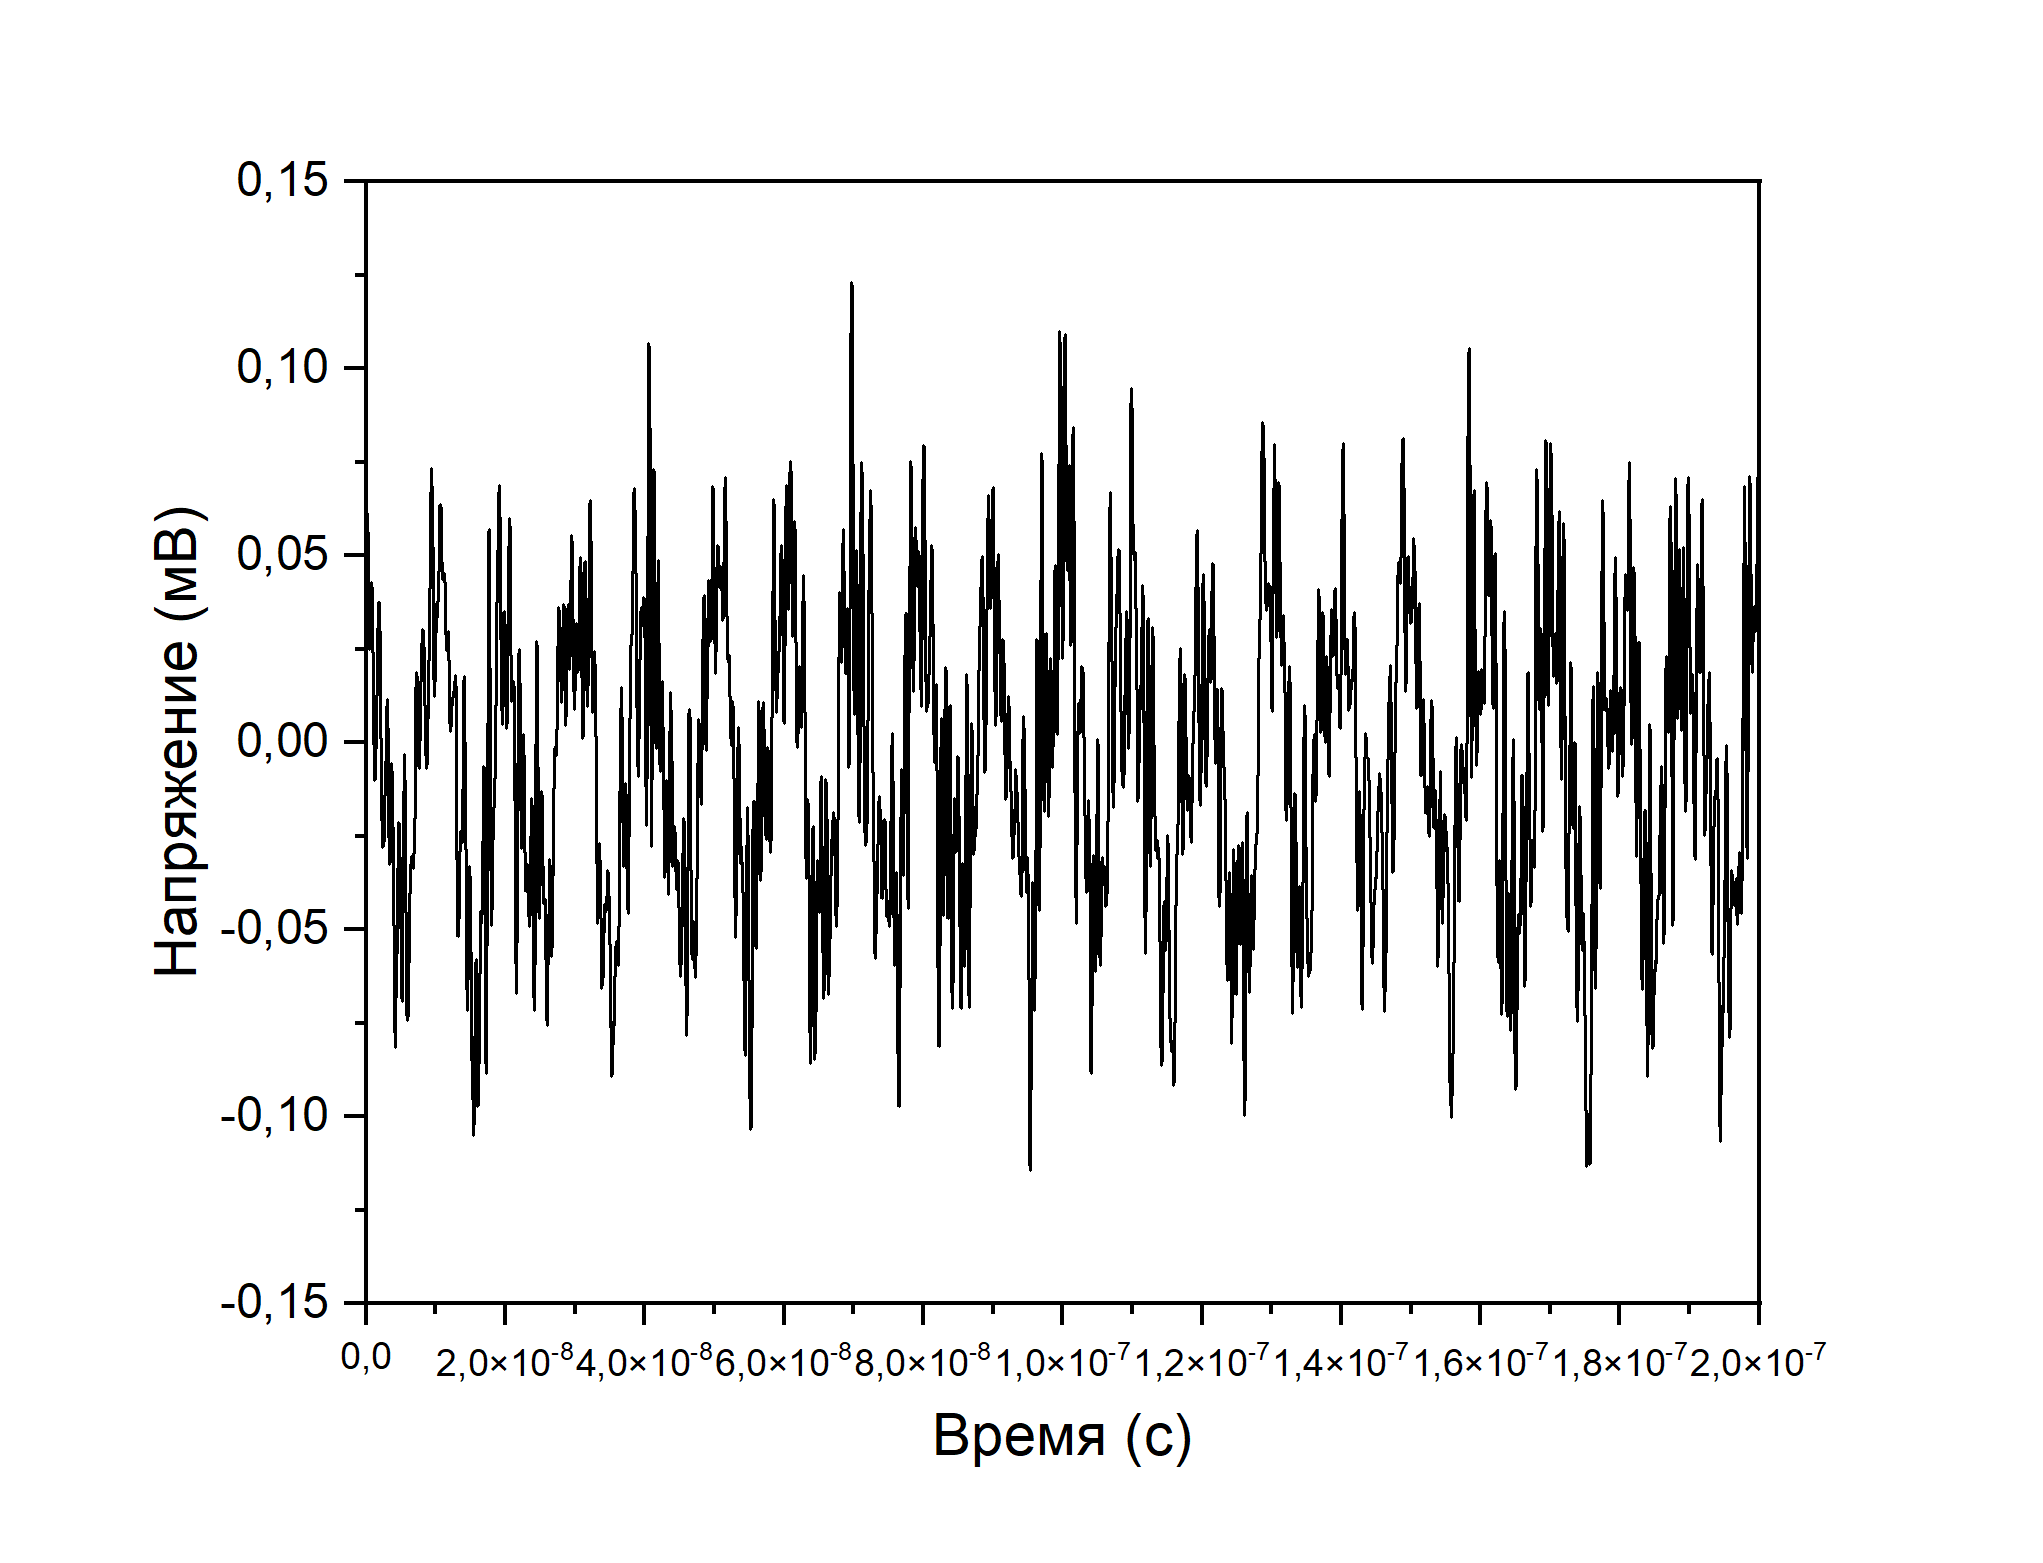
\includegraphics[width=\textwidth]{images/сигнал после бд с новыми шкалами.png}
    \caption{Выходной сигнал балансного детектора после фильтрации.}
    \label{fig:filter 100 mhz ch2}
\end{figure}
После применения к сигналу с рисунка \ref{fig:filter 100 mhz ch2} алгоритма Быстрого Преобразования Фурье для изучения спектрального состава. Результат изображен на рисунке ниже.
\begin{figure}
    \centering
    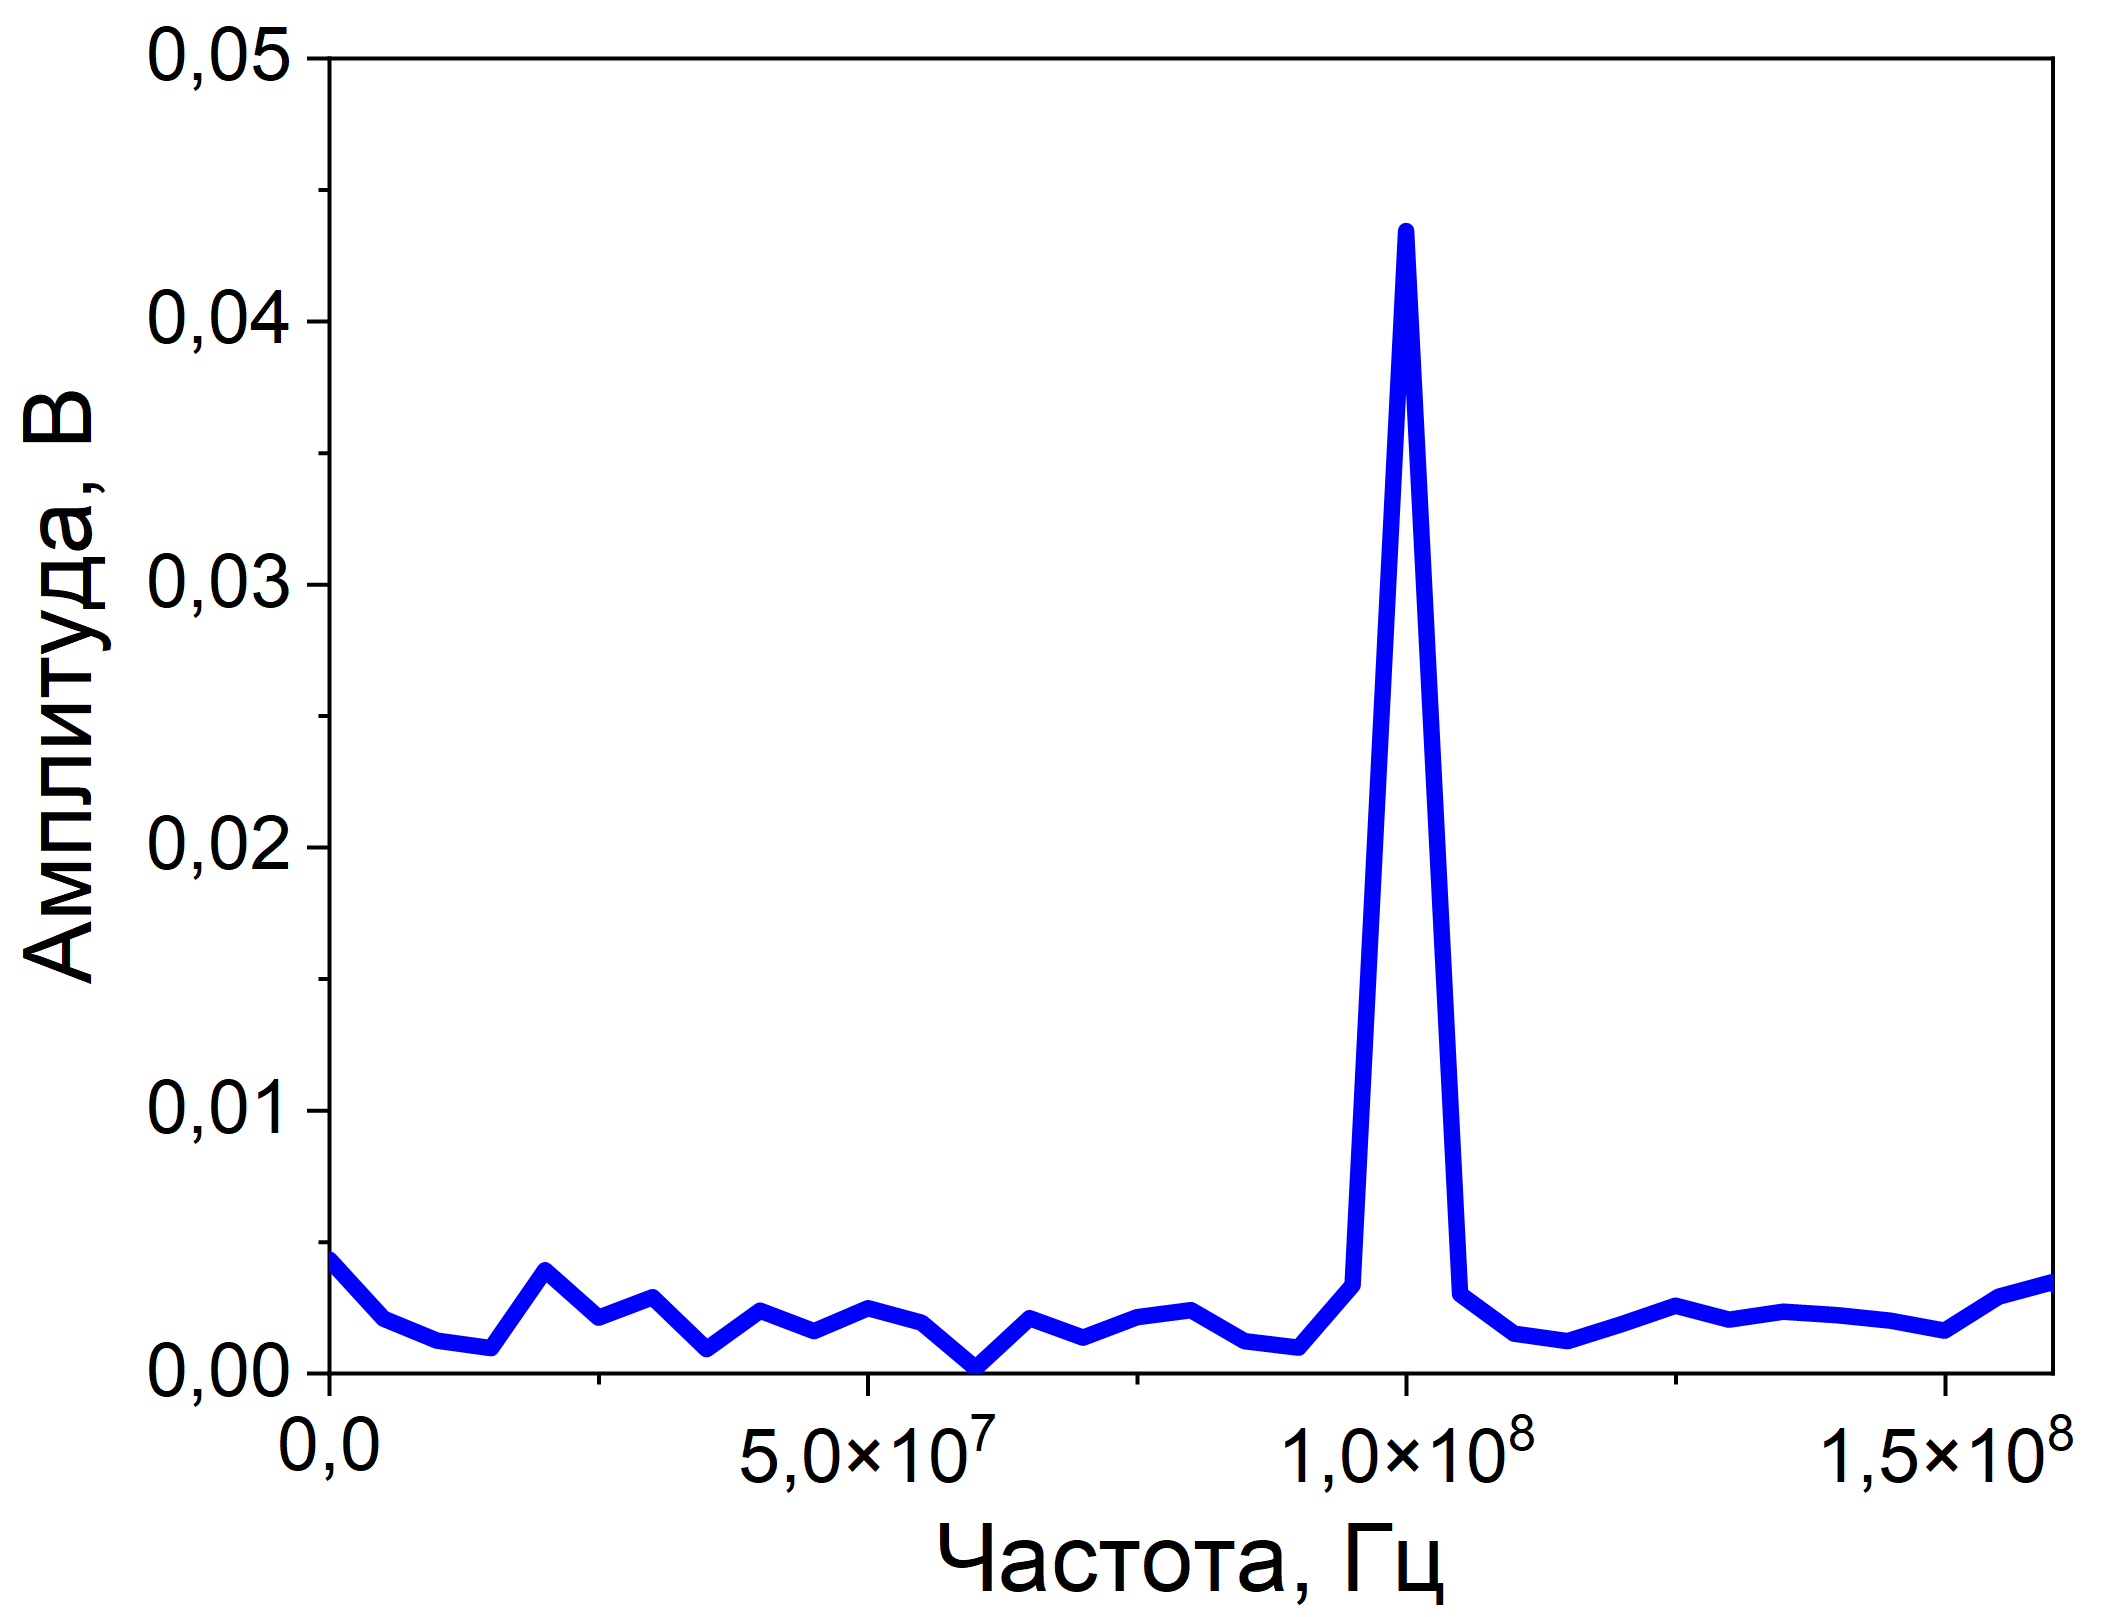
\includegraphics[width=\textwidth]{images/05.png}
    \caption{Спектр полученного сигнала}
    \label{fig:spectrum ch2}
\end{figure}
На рисунке \ref{fig:spectrum ch2} изображен результат БПФ примененноного к сигналу после фильтрации. Единсвтенная гармоника находится на частоте 100 МГц, что согласуется с тем, что частоты лазеров-ведущего и лазера-ведомого совпадают.
Для получения информации о фазе принятого сигнала необходимо цифровыми методами обработки информации извлечь ее оттуда. Для этого также возможно использование быстрого преобразования Фурье. Результат этого преобразования отображен на рисунке \ref{fig:phase meas ch2} 
\begin{figure}
    \centering
    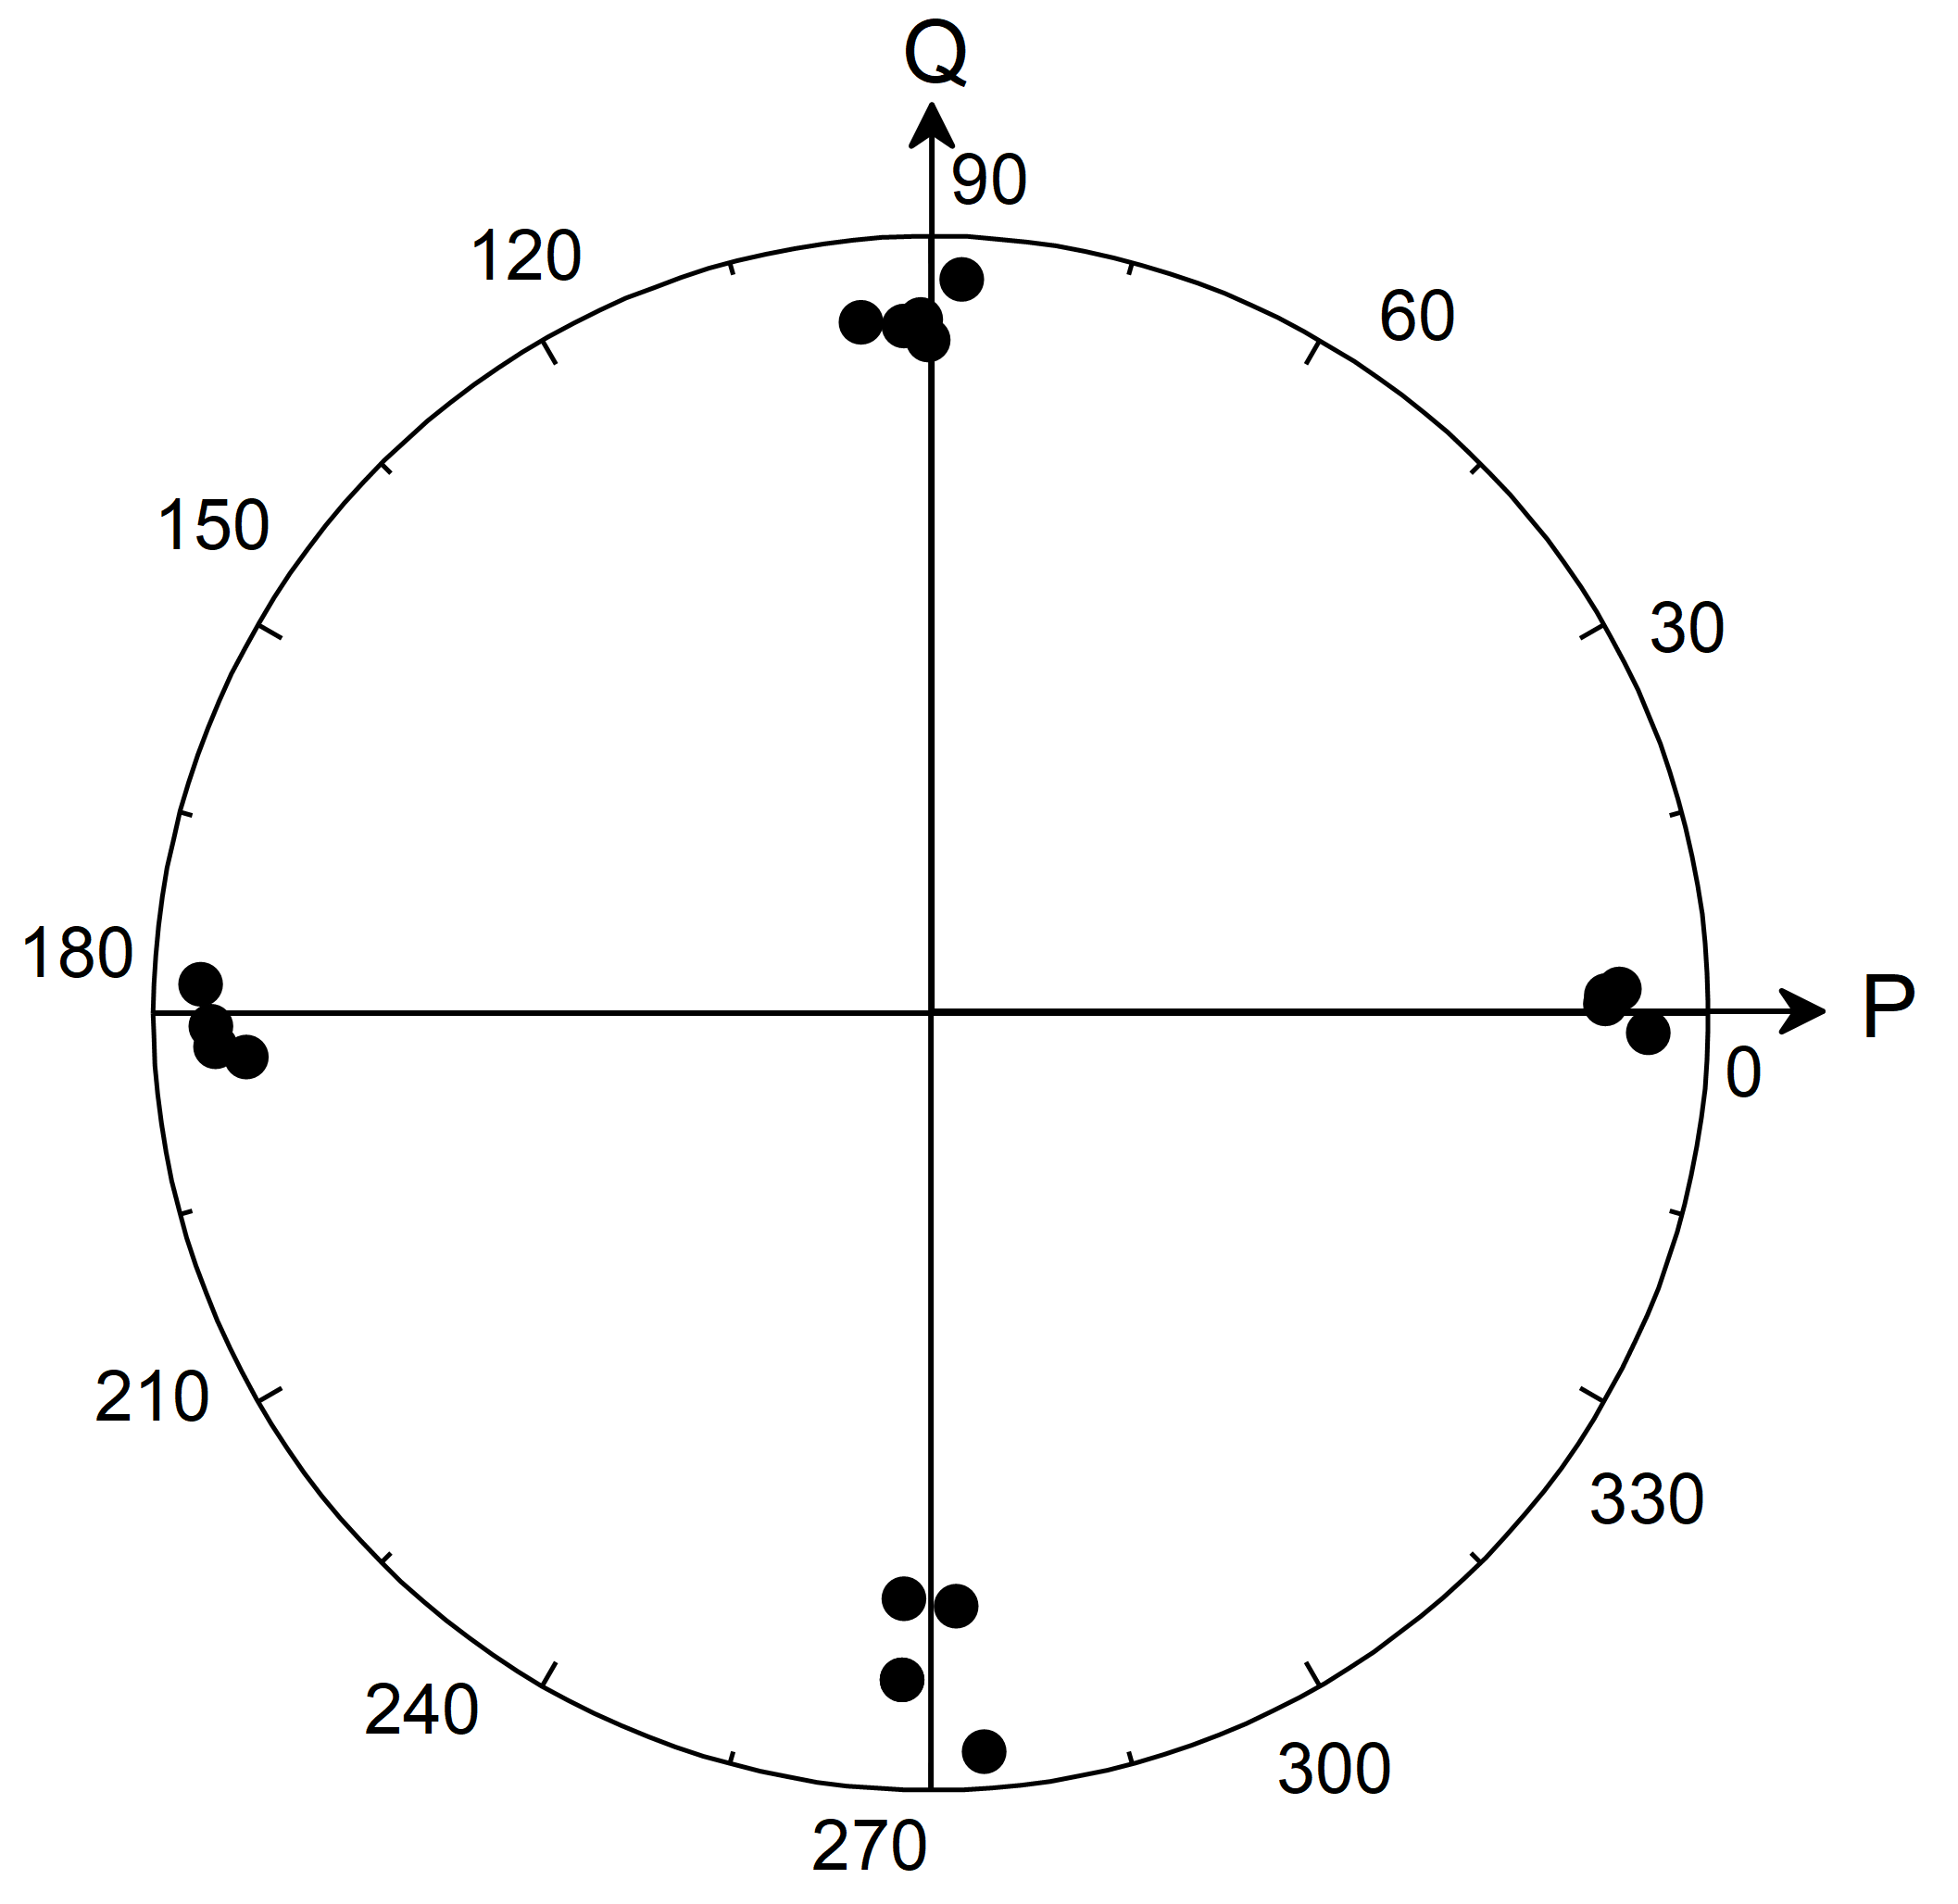
\includegraphics[width=0.7\textwidth]{images/06.png}
    \caption{Измеренные значения фазовых свдигов в выходном сигнале балансного детектора}
    \label{fig:phase meas ch2}
\end{figure}
Для измерения влияния оптической инжекции на длину волны лазера локального осциллятора, установленного на приемной стороне, необходимо измерить длину волны под действием оптической инжекции и без нее. 

\section{Определение фазового шума}\label{sec:ch2/sect6}
\section{Выводы по главе}\label{sec:ch2/sect7}
